\section{Frontend Implementation}
\label{sec:frontend_implementation}

The Candidate Platform's frontend is built on a decoupled architecture, using Drupal 10 as a headless CMS and Next.js 13+ for the user interface \cite{newman2015building}. This setup separates content management from presentation, making the system more flexible and maintainable. The integration relies on JSON:API \cite{dries2019headless}, which exposes all backend data as RESTful endpoints, so there's no need to write custom APIs for every entity or field.

\subsection{Decoupled Architecture and Backend Integration}

The frontend consumes data from Drupal's JSON:API endpoints. Each content type, taxonomy, user, and webform is available as a resource. This approach keeps the backend and frontend loosely coupled, allowing each to evolve independently. The main benefits: faster page loads, easier updates, and a clear separation of concerns.

\subsubsection{JSON:API Integration}

All CRUD operations and relationships are handled through JSON:API. Filtering, sorting, and pagination are built in. For example, fetching a candidate's application and related quiz results or challenge submissions is a single request.

\subsubsection{Widget-Based Content Delivery}
\noindent
A central innovation in the platform is the widget system, which bridges Drupal's content management capabilities with Next.js's component-based rendering. Each widget encapsulates a reusable content component, configurable via Drupal's administrative interface and rendered dynamically on the frontend.

The widget architecture comprises three principal elements:

\begin{enumerate}
    \item \textbf{Backend Widget Configuration}: Widgets are defined in Drupal using \texttt{settings.yml} files, specifying JSON:API queries, field filters, and sorting logic.
    \item \textbf{Frontend Widget Components}: React components that receive and render data provided by the backend.
    \item \textbf{Webpack Build-Time Mapping}: An automated system that maps backend widget configurations to their corresponding frontend components during the build process and inject the data into the components.
\end{enumerate}

\subsubsection{Webpack Plugin Architecture}
\noindent
The mapping between backend widget configurations and frontend components is orchestrated by a custom Webpack plugin. This plugin automates the discovery and registration of widget components, ensuring seamless integration and maintainability. The core responsibilities of the \texttt{WidgetsPlugin} include:

\begin{enumerate}
    \item \textbf{Component Discovery}: Scanning the codebase for files matching the \texttt{*Widget.jsx} and \texttt{*Node.jsx} pattern.
    \item \textbf{Configuration Extraction}: Parsing each component's \texttt{config.id} to establish unique identifiers.
    \item \textbf{Dynamic Import Generation}: Supporting both lazy and direct imports for optimal performance.
    \item \textbf{Mapping File Creation}: Generating a mapping file (\texttt{widgets.js}) that links widget IDs to their respective components.
\end{enumerate}

% The complete implementation of the Webpack plugin is provided in Appendix~\ref{appendix:webpack_plugin}.

\begin{figure}[H]
    \centering
    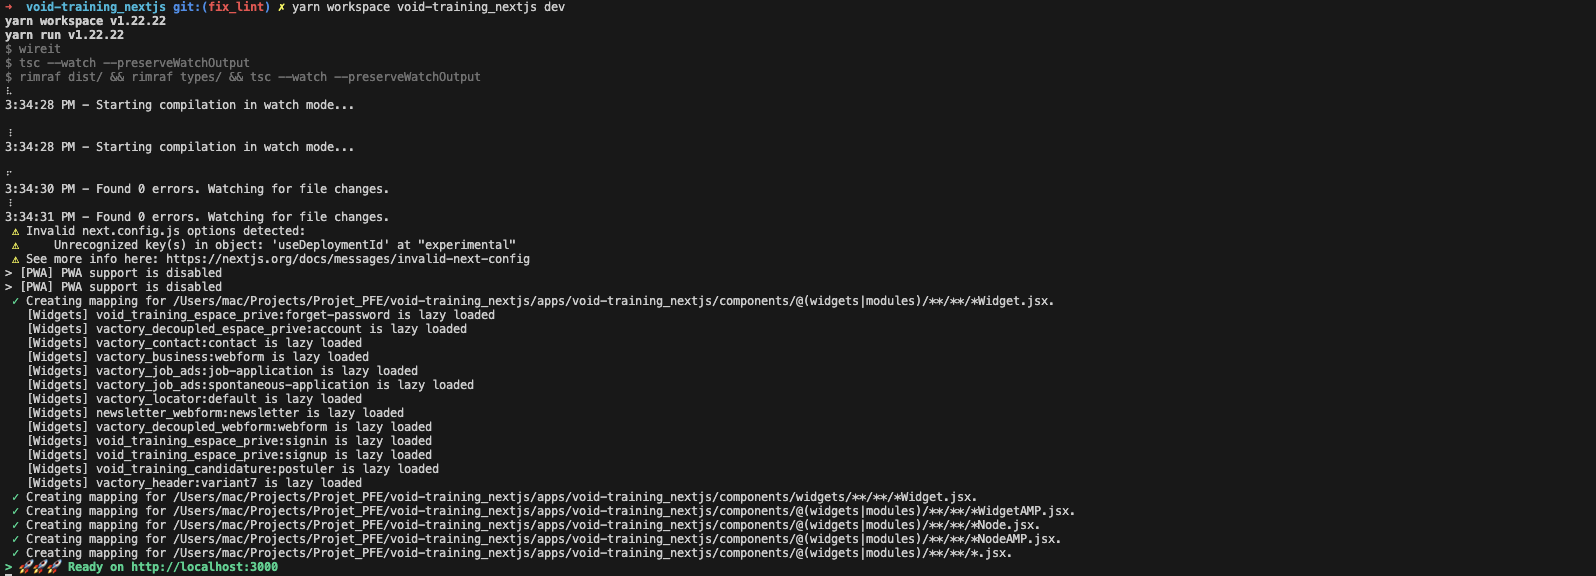
\includegraphics[width=\textwidth]{images/webpack_mapping.png}
    \caption{Webpack Mapping Process}
    \label{fig:webpack_mapping}
\end{figure}

\begin{figure}[H]
    \centering
    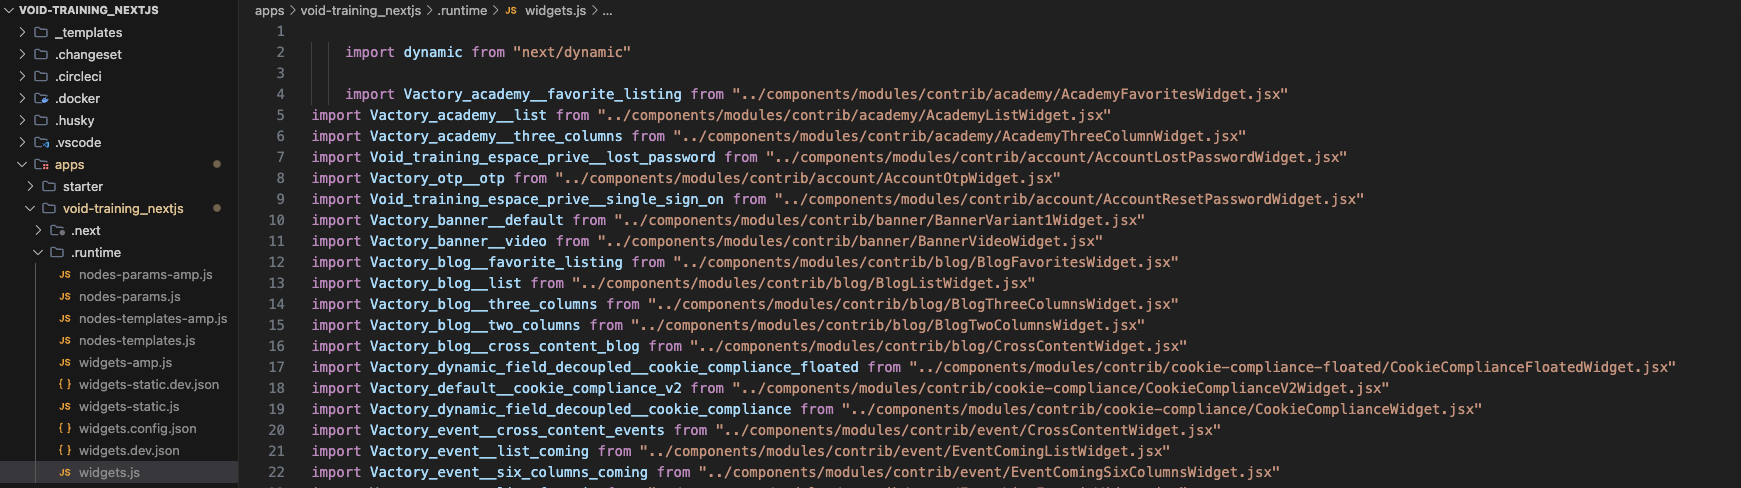
\includegraphics[width=\textwidth]{images/webpack_listing.png}
    \caption{Webpack Listing File}
    \label{fig:webpack_listing}
\end{figure}

\subsection{Routing and Path Resolution}

\subsubsection{Slug-Based Routing}
\noindent
The frontend employs a catch-all route pattern (\texttt{[...slug].jsx}) to intercept and process all navigation requests. The routing workflow is as follows:

\begin{enumerate}
    \item \textbf{Path Translation}: The frontend transmits the requested path to Drupal's translate route endpoint.
    \item \textbf{UUID Resolution}: The Pathauto module resolves the alias to the corresponding content UUID.
    \item \textbf{Content Fetching}: The UUID is used to retrieve the full content entity via JSON:API.
    \item \textbf{Component Rendering}: The retrieved content is passed to the appropriate page template for rendering.
    \item \textbf{UUID Caching}: The UUID is cached in redis to avoid unnecessary API calls.
\end{enumerate}



\subsubsection{API Proxy Implementation}
\noindent
To further abstract backend infrastructure and enhance security, all API requests from the frontend are routed through a Next.js API proxy. This proxy is responsible for authentication, caching, and forwarding requests, thereby maintaining a clear separation of concerns.

Key features of the proxy include:

\begin{itemize}
    \item \textbf{URL Rewriting}: Requests to \texttt{/api/proxy/*} are transparently forwarded to the Drupal backend.
    \item \textbf{Response Caching}: GET requests are cached using Redis to improve performance and reduce backend load.
    \item \textbf{Header Management}: Authentication and other headers are managed and forwarded as required.
    \item \textbf{Error Handling}: Robust error handling ensures appropriate HTTP status codes and user feedback.
\end{itemize}

\subsection{Monorepo Architecture and Starter Kit Integration}
\noindent
The project is structured as a monorepo, promoting code reuse and consistency across platform components. The monorepo is anchored by the Vactory starter kit, which provides foundational components and utilities.

\subsubsection{Workspace Organization}
\noindent
The monorepo is organized into distinct workspaces, each serving a specific function:

\begin{enumerate}
    \item \textbf{Vactory Starter Kit}: Contains core components, utilities, and design system elements.
    \item \textbf{Project Workspace}: Houses custom components and modules specific to the intern management platform.
    \item \textbf{Shared Dependencies}: Centralized configuration for linting, TypeScript, and other shared tooling.
\end{enumerate}

A schematic of the directory structure is provided below:

\begin{verbatim}[caption={Monorepo Directory Structure}, captionpos=b]
void-training_nextjs/
├── packages/
│   └── core/
│   └── console/
├── apps/
│   └── starter/ # Vactory starter kit that is synchronized with the Vactory starter kit repository
│   └── void-training_nextjs/
│       ├── .next/
│       ├── .storybook/
│       ├── hooks/
│       ├── lib/
│       ├── pages/
│       ├── public/
│       ├── components/
│       │   ├── elements/          # Atomic components
│       │   ├── widgets/           # Content widgets
│       │   └── modules/           # Complex modules
│       ├── pages/
│       └── public/
└── shared/
    ├── eslint-config/
    └── typescript-config/
\end{verbatim}

\subsection{Design System and Storybook Integration}

Storybook is central to our design system. It lets us build and test UI components in isolation, document usage, and share previews with stakeholders. Each component has stories showing its different states and props. The Button component, for example, is documented with all its variants and sizes.

\begin{figure}[H]
    \centering
    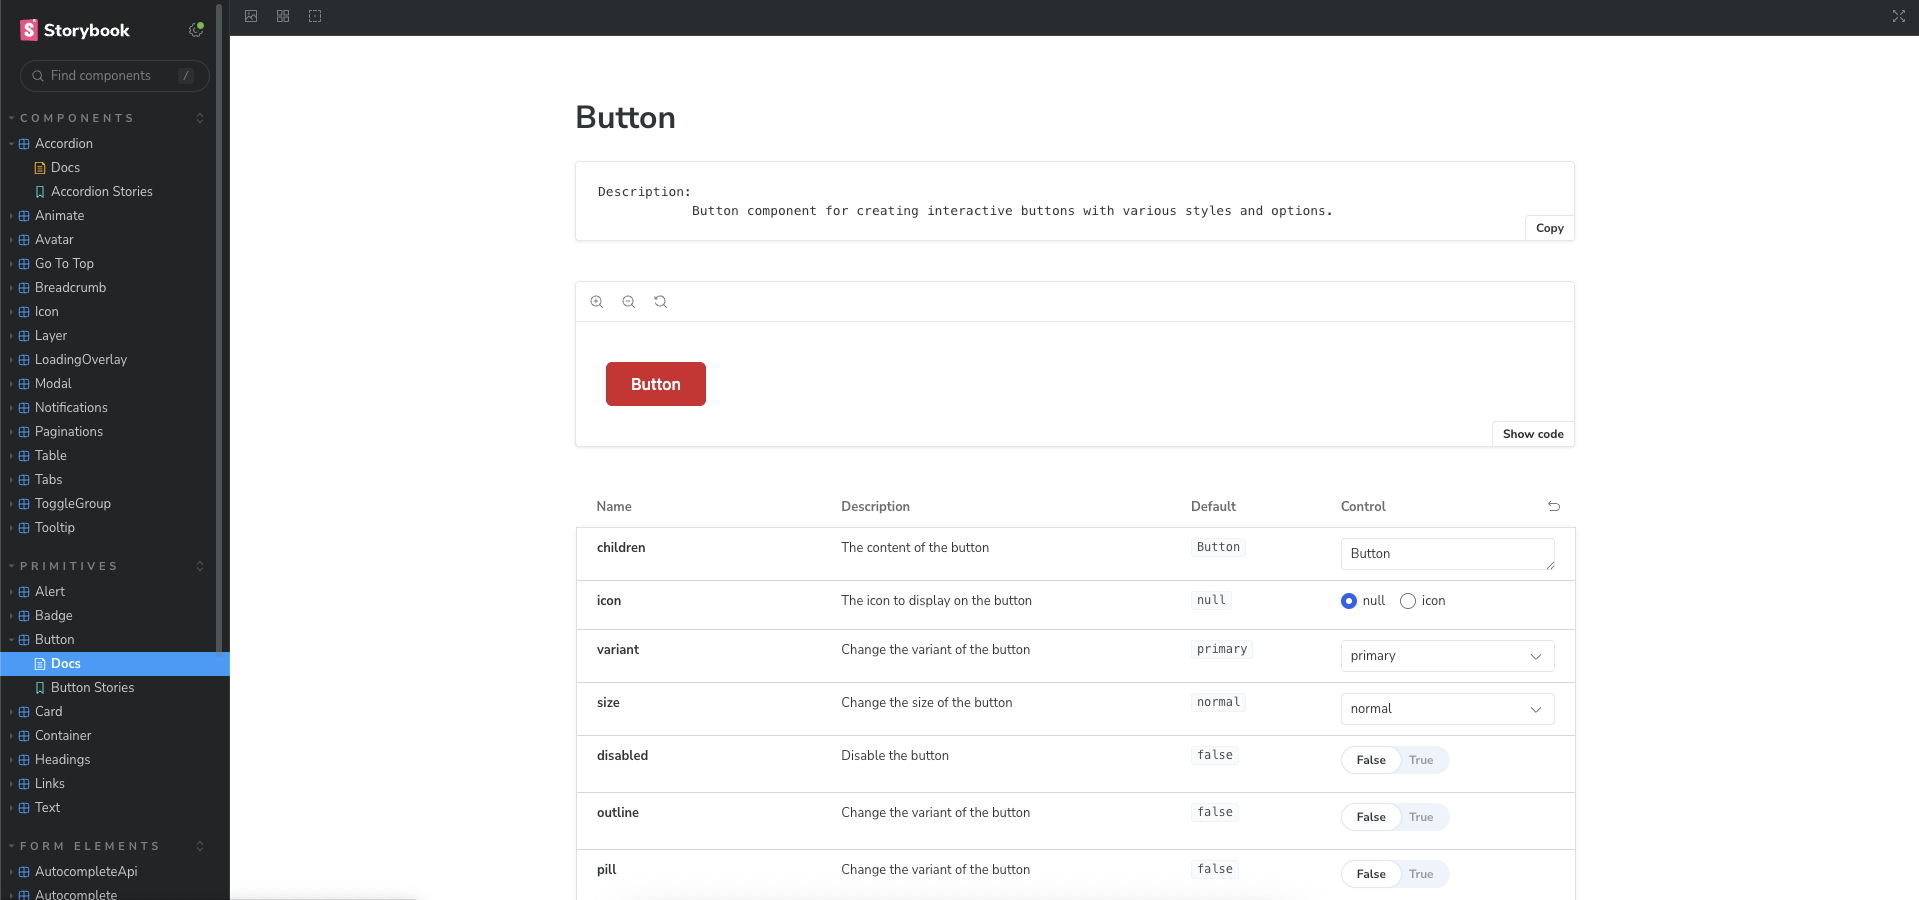
\includegraphics[width=\textwidth]{images/storybook_button.png}
    \caption{Storybook Button Component}
    \label{fig:storybook_button}
\end{figure}

\subsection{Icon System and Asset Management}

Icons are managed as an SVG sprite, generated at build time. This keeps asset delivery efficient and usage flexible. The build script optimizes SVGs, tidies up the code, and aggregates everything into a single sprite in the public directory.

\begin{lstlisting}[caption={Icon Build Script Configuration}, captionpos=b]
{
  "scripts": {
    "icons:build": "npx --yes @vactorynext/svg-spreact-cli ./icons --optimize true --tidy true > ./public/icons.svg"
  }
}
\end{lstlisting}

This process encompasses:

\begin{itemize}
    \item \textbf{SVG Optimization}: Removal of extraneous metadata and path optimization.
    \item \textbf{Code Tidying}: Cleanup of SVG markup for minimal file size.
    \item \textbf{Sprite Generation}: Aggregation of all icons into a single sprite file.
    \item \textbf{Public Exposure}: Placement of the sprite in the public directory for direct access.
\end{itemize}


\subsection{Custom Widgets and Modules Implementation}

Custom widgets and modules power both content presentation and interactive features. The platform implements two main categories of widgets:

\textbf{Core Layout Widgets}
\begin{itemize}
    \item \textbf{Header Widget}: Implements the site's navigation structure with:
    \begin{itemize}
        \item Main menu integration
        \item User authentication status
        \item Responsive mobile menu
    \end{itemize}
    
    \item \textbf{Footer Widget}: Provides site-wide footer content including:
    \begin{itemize}
        \item Company information
        \item Social media links
        \item Quick navigation links
    \end{itemize}
    
    \item \textbf{Hero Widget}: Creates impactful landing sections with:
    \begin{itemize}
        \item Background image/video support
        \item Call-to-action buttons
        \item Customizable text content
    \end{itemize}
\end{itemize}

\textbf{Content Display Widgets}
\begin{itemize}
    \item \textbf{Card Listing Widgets}:
    \begin{itemize}
        \item \textbf{Tagged Cards}: Displays content cards with taxonomy term filters
        \item \textbf{Duration Cards}: Shows cards with time-based labels (e.g., "2 weeks", "3 months")
        \item \textbf{Numbered Cards}: Presents content in a numbered sequence
    \end{itemize}
    
    \item \textbf{Testimonial Widget}: Showcases user feedback with:
    \begin{itemize}
        \item User profile information
        \item Rating system
        \item Quote content
        \item Optional profile images
    \end{itemize}

    \item \textbf{Slider Widget}: Creates dynamic content carousels with:
    \begin{itemize}
        \item Auto-play and manual navigation controls
        \item Responsive image optimization
        \item Custom transition effects
        \item Mobile-friendly touch gestures
    \end{itemize}

    \item \textbf{Project Showcase Widget}: Displays past intern projects with:
    \begin{itemize}
        \item Project title and description
        \item Technologies used (with icons)
        \item Project duration and completion date
        \item Link to project repository or demo
        \item Intern's name and role
    \end{itemize}
\end{itemize}



% \subsubsection{Candidate Tracking Implementation}
% \noindent
% The candidate tracking module is particularly noteworthy for its complexity and user-centric design. It provides a comprehensive overview of the application process, dynamically updating status and available actions:

% \begin{lstlisting}[caption={Candidate Tracking Widget Structure}, captionpos=b]
% export const config = {
%     id: "void_training_candidature:suivi",
% };
% const CandidatSuiviWidget = ({ data }) => {
%     const { profile } = useAccount();
%     const currentStatus = profile?.user?.candidature?.status;
%     //render the data coming from drupal
% };
% \end{lstlisting}

% \subsection{Context-Based Candidature Data}

% React Context manages global state for candidature data. This avoids prop drilling and keeps state accessible across deeply nested components.
% \subsection{React Query Integration}

% React Query handles server state, caching, and background updates. Custom hooks fetch candidature data, submit quizzes, and manage mutations. This setup keeps the UI responsive and data fresh, even with multiple users and frequent updates.


\subsection{Performance Optimization and Testing}
\noindent
Performance and reliability are ensured through a combination of optimization techniques and rigorous testing.

\subsubsection{Redis Integration for Performance Optimization}
\noindent
Redis and Redis Commander play a crucial role in optimizing the platform's performance through efficient caching mechanisms. Redis serves as an in-memory data structure store, while Redis Commander provides a web interface for managing Redis instances.

The integration of Redis in our project serves several key purposes:

\begin{enumerate}
    \item \textbf{API Response Caching}: Redis caches JSON:API responses from Drupal, significantly reducing response times for frequently accessed data.
    \item \textbf{Session Management}: User sessions and authentication tokens are stored in Redis, enabling fast retrieval and validation.
    \item \textbf{Rate Limiting}: Redis helps implement rate limiting for API endpoints, preventing abuse and ensuring system stability.
    \item \textbf{Real-time Updates}: Redis pub/sub functionality enables real-time updates for features like quiz submissions and status changes.
    \item \textbf{Offline Mode Support}: Redis caches enable offline functionality when the backend is unavailable.
\end{enumerate}

Redis Commander is utilized for:
\begin{enumerate}
    \item \textbf{Monitoring}: Real-time visualization of Redis operations and memory usage.
    \item \textbf{Data Management}: Easy inspection and modification of cached data.
    \item \textbf{Performance Analysis}: Tracking cache hit rates and response times.
    \item \textbf{Debugging}: Quick access to cached content for troubleshooting.
\end{enumerate}

\begin{figure}[H]
    \centering
    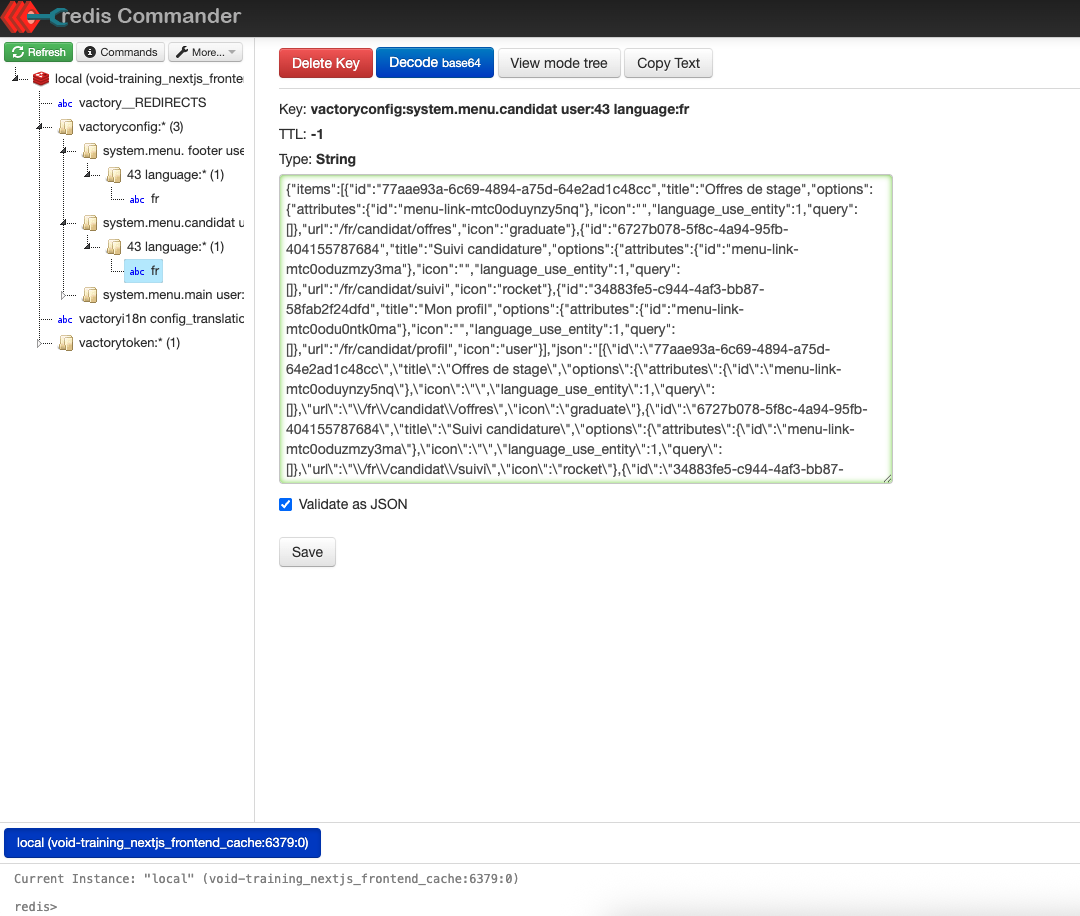
\includegraphics[width=\textwidth]{images/redisCommander.png}
    \caption{Redis Commander UI}
    \label{fig:redis_commander}
\end{figure}

\subsubsection{Offline Mode Implementation}
\noindent
A critical feature of our platform is the offline mode capability, which ensures users can access content even when the backend is unavailable or there's no internet connection. This functionality leverages Redis caching to maintain platform availability during service interruptions.

When offline mode is enabled, the system operates as follows:

\begin{enumerate}
    \item \textbf{Cache Detection}: The frontend detects when the backend API is unreachable through failed request monitoring.
    \item \textbf{Redis Fallback}: Instead of displaying error messages, the system automatically switches to serve cached content from Redis.
    \item \textbf{Content Delivery}: Users continue to access previously cached pages, widgets, and essential platform functionality.
    \item \textbf{User Notification}: A subtle indicator informs users they're viewing cached content in offline mode.
    \item \textbf{Automatic Recovery}: When backend connectivity is restored, the system seamlessly transitions back to live data.
\end{enumerate}

\begin{figure}[H]
    \centering
    \makebox[\textwidth]{%
        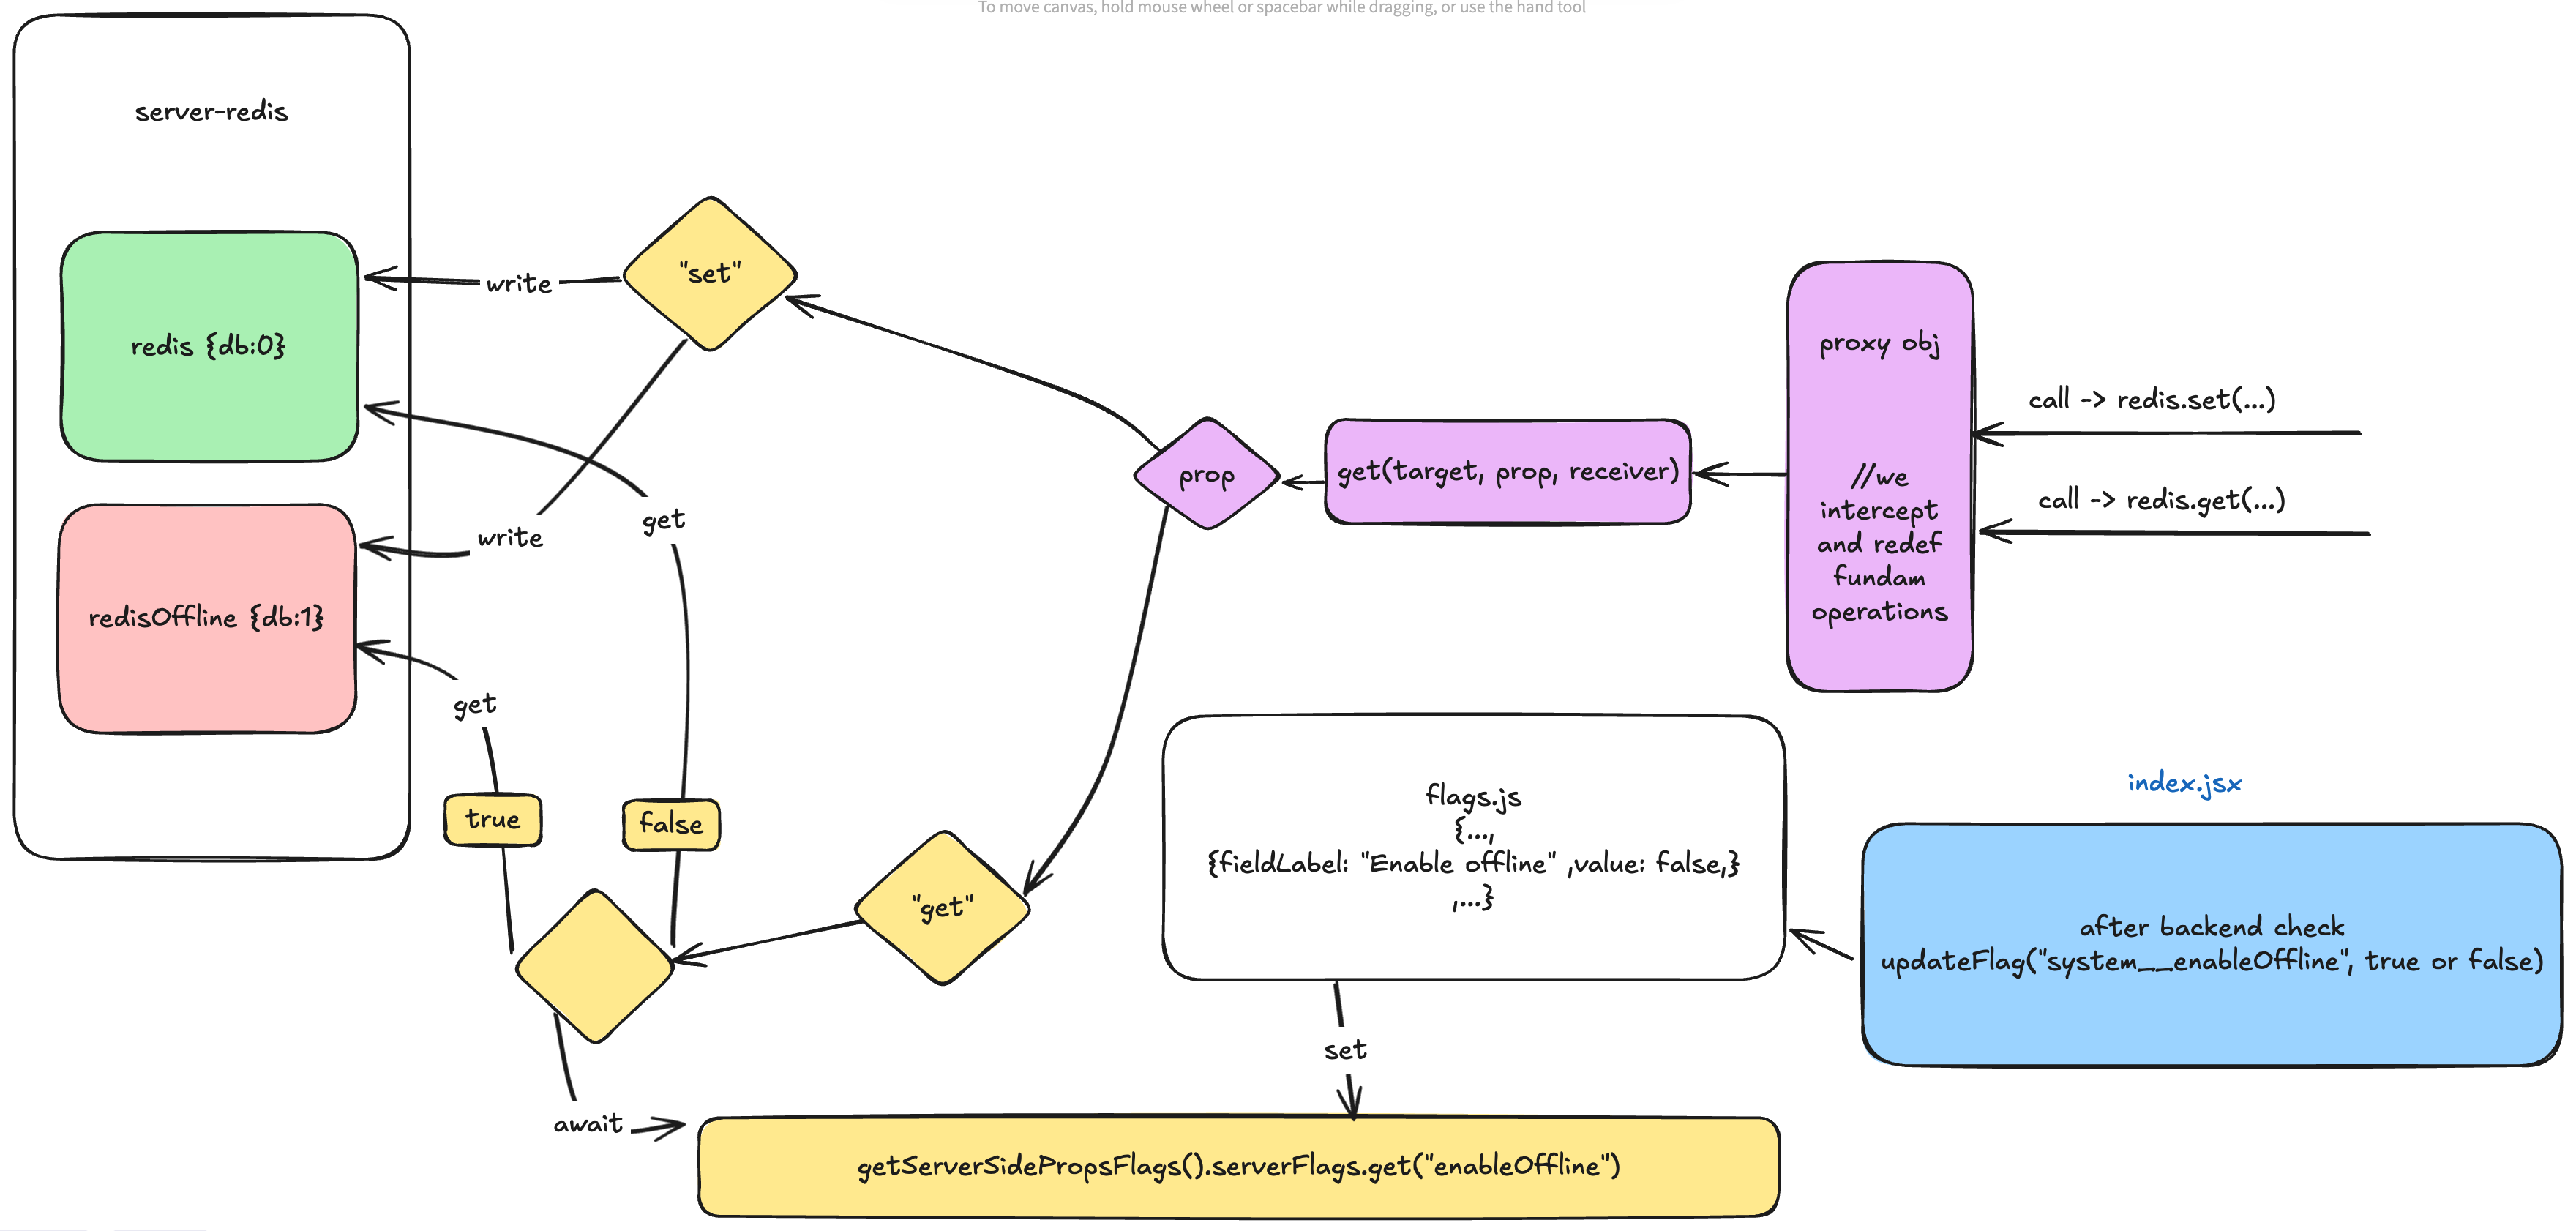
\includegraphics[width=1.1\textwidth]{images/Screenshot-offline.png}%
    }
    \caption{Offline Mode Implementation with Redis Cache Schema}
    \label{fig:offline_mode_sequence}
\end{figure}

This approach ensures business continuity and maintains user experience quality even during technical difficulties or maintenance windows. Candidates can still access their application status, view job offers, and navigate the platform when the backend is temporarily unavailable.

% The complete offline mode implementation is detailed in Appendix~\ref{appendix:offline_mode}.

The frontend is designed for maintainability, scalability, and a smooth user experience. Decoupled architecture, component-driven design, and robust state management keep the platform flexible and ready for future growth.
